\documentclass{standalone}

\usepackage{amsmath,amsfonts,amssymb,amsthm,mathtools} 
\usepackage{fontspec}            % пакет для подгрузки шрифтов
\setmainfont{Amiri}   % задаёт основной шрифт документа

% why do we need \newfontfamily:
% http://tex.stackexchange.com/questions/91507/
\newfontfamily{\cyrillicfonttt}{Amiri}
\newfontfamily{\cyrillicfont}{Amiri}
\newfontfamily{\cyrillicfontsf}{Burst My Bubble}
% Иногда тех не видит структуры шрифтов. Эти трое бравых парней спасают ситуацию и доопределяют те куски, которые Тех не увидел.

\usepackage{unicode-math}     % пакет для установки математического шрифта
\setmathfont{Asana Math}      % шрифт для математики

\usepackage{polyglossia}      % Пакет, который позволяет подгружать русские буквы
\setdefaultlanguage{russian}  % Основной язык документа
\setotherlanguage{english}    % Второстепенный язык документа

\usepackage{pgf,tikz,pgfplots}
\usetikzlibrary{arrows,calc}
\usepackage{relsize} 

\usepackage{graphicx} 
\usepackage{rotating}
\usepackage{xcolor}
\usepackage{color}

\definecolor{gitt}{HTML}{713015}

\begin{document}

\begin{tikzpicture}[
        scale=2,
        dot/.style={circle,fill=black,minimum size=4pt,inner sep=0pt,
            outer sep=-1pt},
    ]
    
\begin{scope}[rotate=30]       
% Radius of regular polygons
  \newdimen\R
  \R=2cm
  \coordinate (center) at (0,0);
 \draw (0:\R)
     \foreach \x in {60,120,...,360} {  -- (\x:\R) }
              -- cycle (300:\R)
              -- cycle (240:\R)
              -- cycle (180:\R)
              -- cycle (120:\R)
              -- cycle (60:\R)
              -- cycle (0:\R)  [line width=1.9mm,color=gitt,fill=white,fill opacity=0];
\end{scope}
           
              
\begin{scope}[yshift=0cm]              
% beta-coef     
\node[inner sep=0pt,scale=12] (russell) at (0,0){$\hat{\mupbeta}$};   
% left hand
\draw (0.4,0.4) .. controls (0.6,-0.5) and (0.6,-0.5) .. (0.6,0) [line width=1.8pt];         
% guitar
\node[inner sep=0pt] (russell) at (-0.07,-0.3){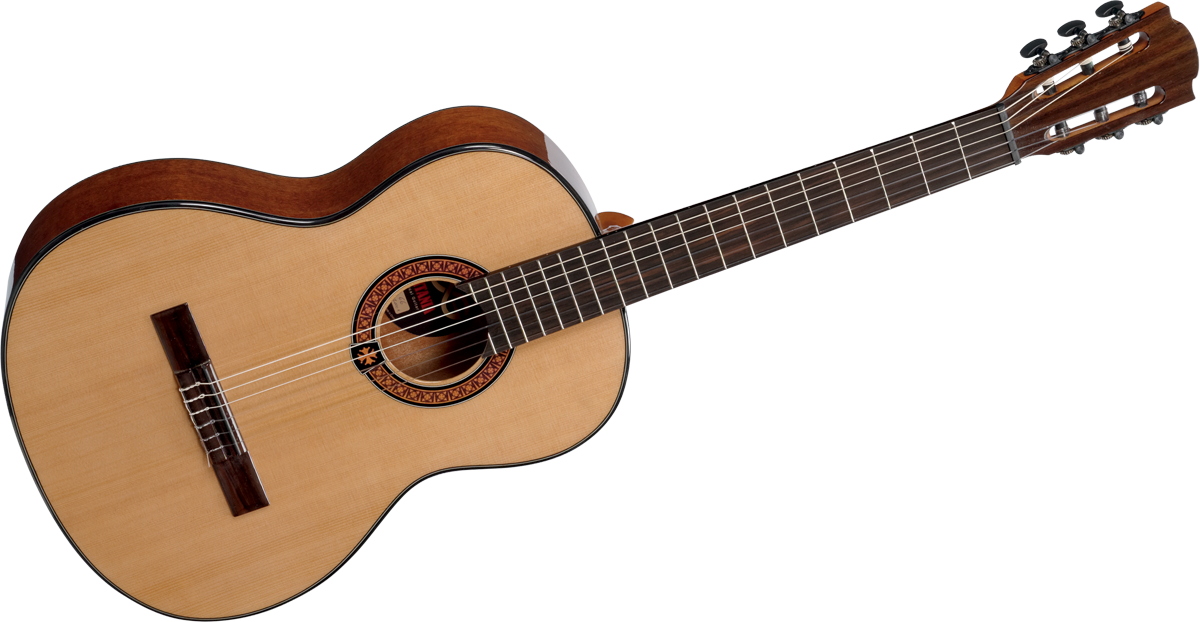
\includegraphics[angle=0,scale=0.12]{git2.png}};        
% right hand
\draw (-0.2,0.2) .. controls (-1,0) and (-1,0) .. (-0.45,-0.4) [line width=1.8pt];
% fingers on the left hand
\draw (0.6,-0.1) -- (0.65,0.055)[line width=1.1pt]; 
\draw (0.6,-0.2) -- (0.6,-0.1)[line width=1.8pt]; 
\draw (0.6,-0.1) -- (0.6,0.055)[line width=1.1pt]; 
\draw (0.6,-0.1) -- (0.55,0.055)[line width=1.1pt]; 
% fingers on the right hand
\draw (-0.45,-0.4) -- (-0.35,-0.45)[line width=1.1pt]; 
\draw (-0.45,-0.4) -- (-0.35,-0.40)[line width=1.1pt]; 
\draw (-0.45,-0.4) -- (-0.38,-0.50)[line width=1.1pt];        
\end{scope}       

\begin{scope}[yshift=-0.9]
% pictures for guitar
\node[inner sep=0pt] (russell) at (-1,-0.8){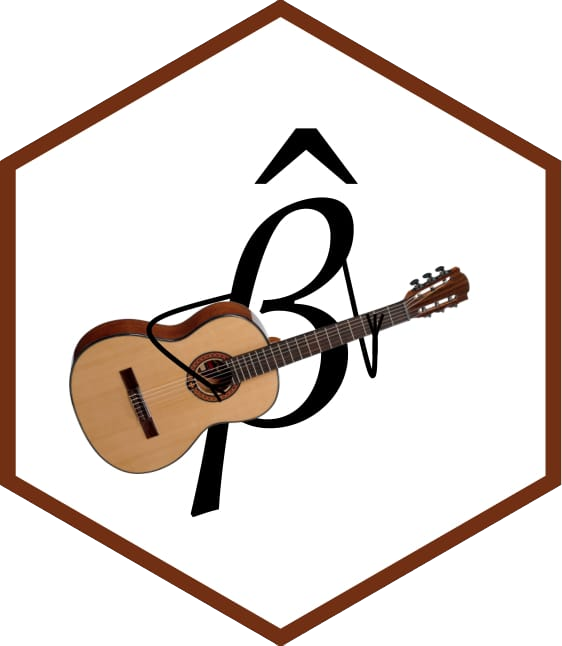
\includegraphics[angle=20,scale=0.0155]{beta-1.png}};
\node[inner sep=0pt] (russell) at (-1.115,-0.702){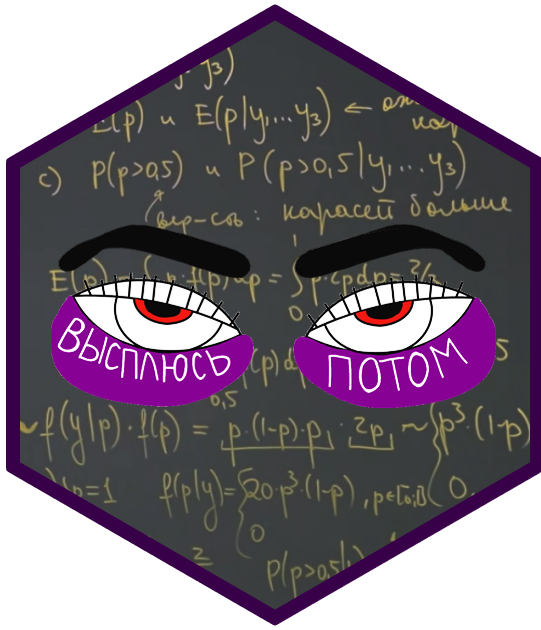
\includegraphics[angle=20,scale=0.0155]{potom_spat.png}};
\node[inner sep=0pt] (russell) at (-0.965,-0.646){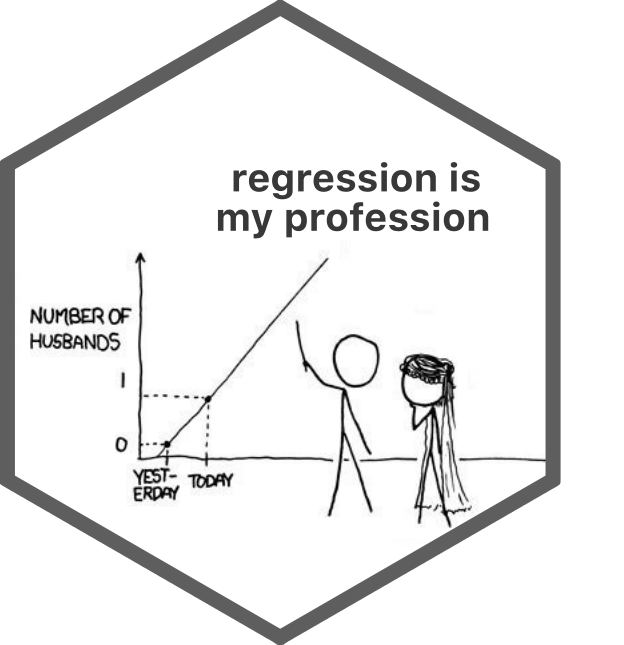
\includegraphics[angle=20,scale=0.0155]{regression_is_my.png}};
\end{scope}

% hat
\node[inner sep=0pt] (russell) at (0.20,0.95){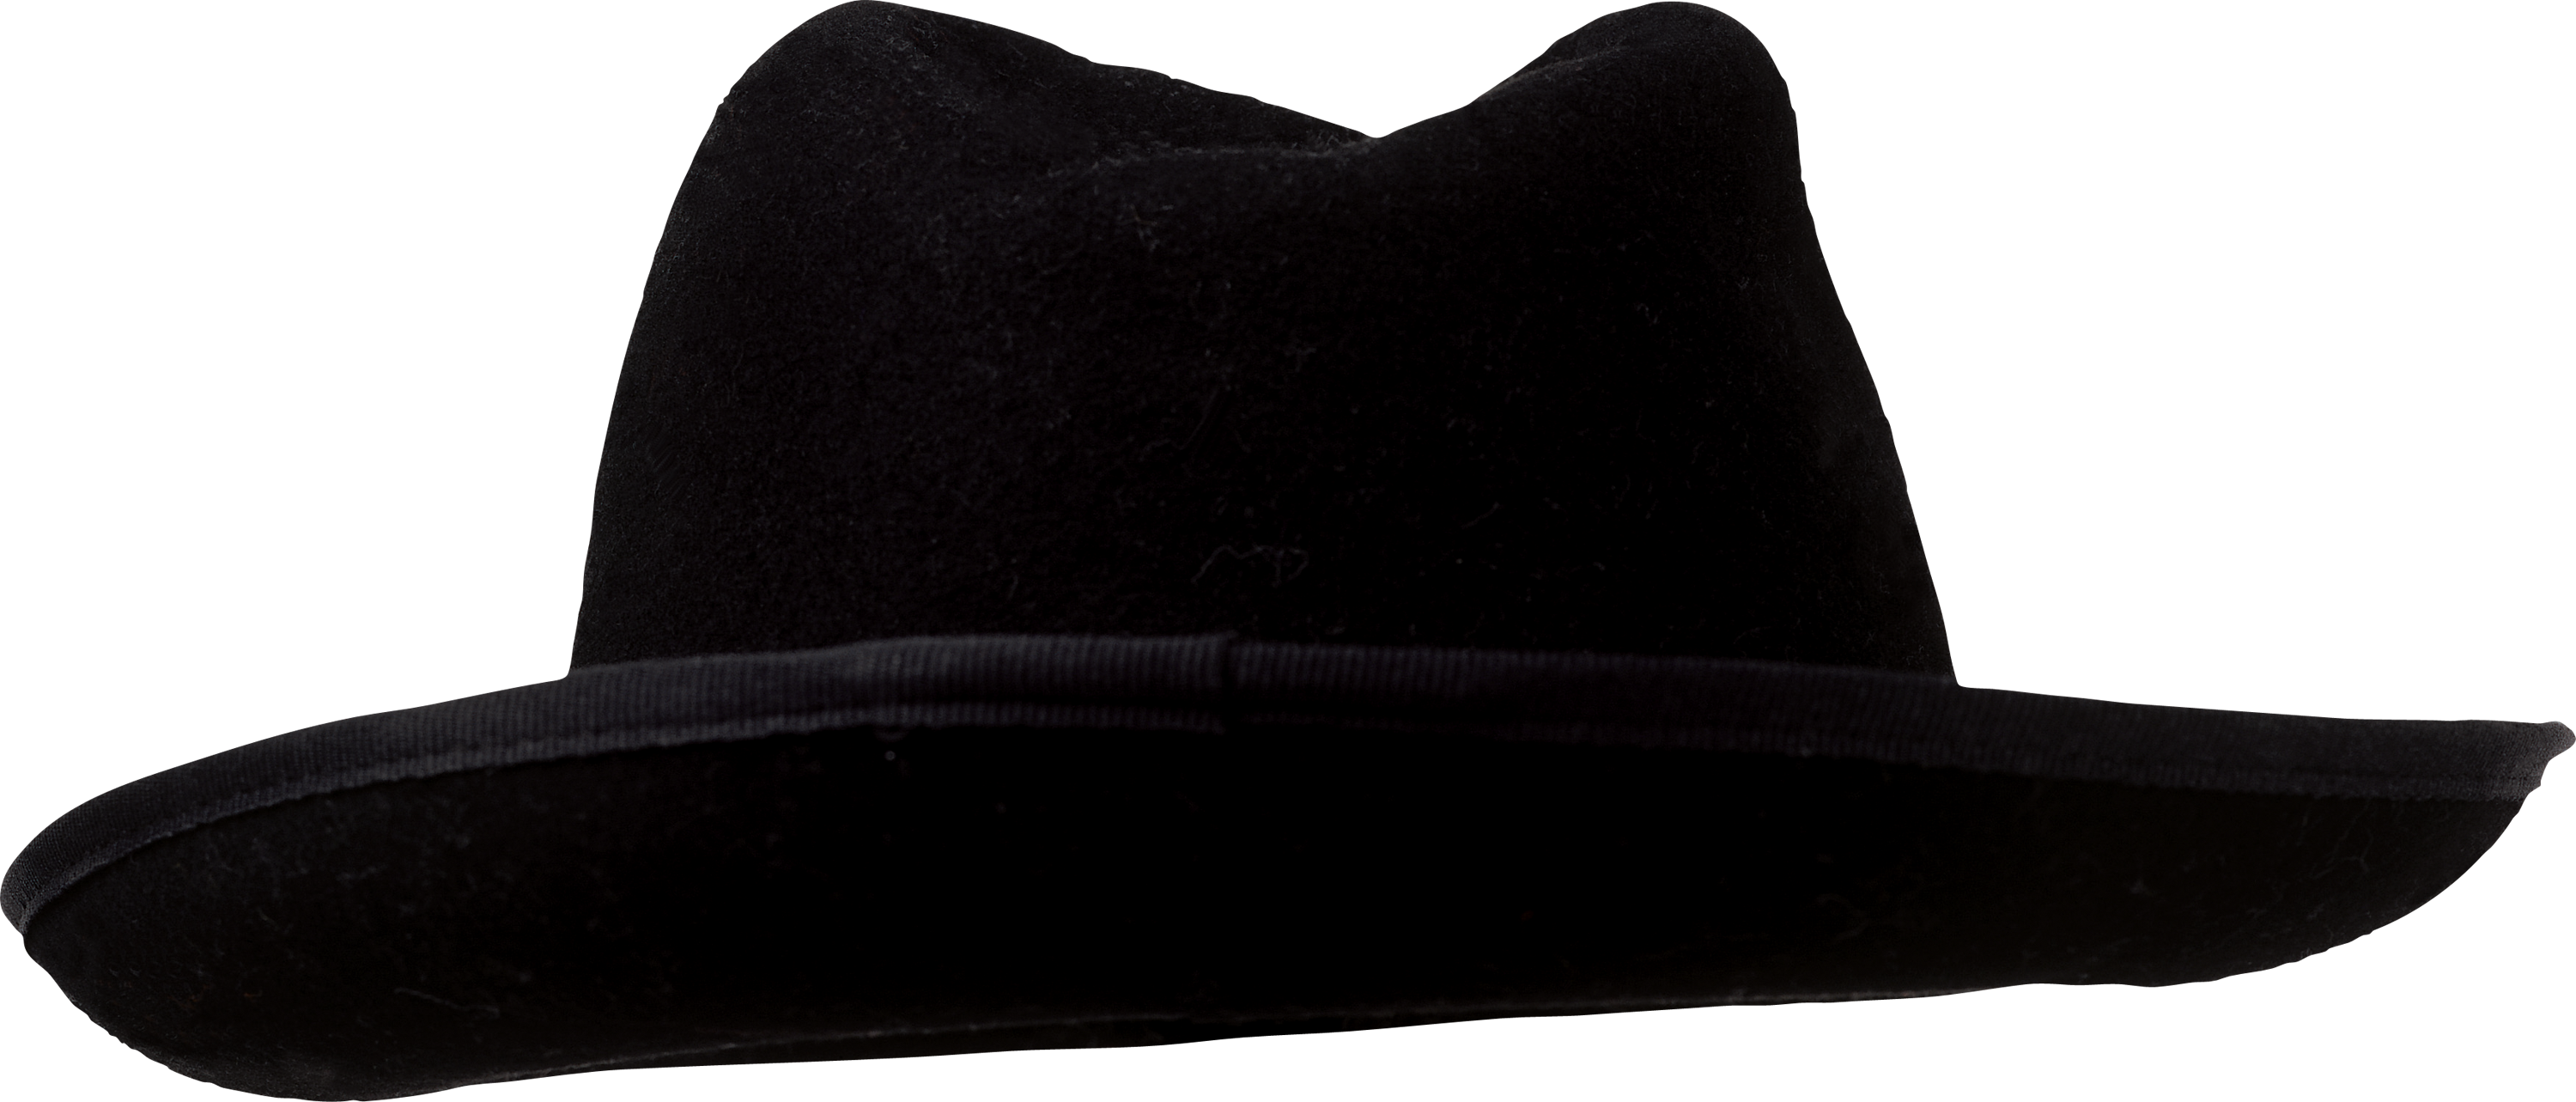
\includegraphics[angle=0,scale=0.125]{hat.png}};        

\draw[color=white,align=left,scale=1.1] (-0.05,0.92) node[right] { \textbf{$1.96$}};
                  
\end{tikzpicture}


\end{document}